\section{Image Restoration}

\subsection{Degradation}

물체에서 반사되거나 발광하는 원본 빛 $f$를 그대로 얻을 수 없음. 다양한 원인으로 노이즈 $\eta$가 더해지고 degradation $h$가 적용된 $g$를 얻게 되기 때문.

노이즈는 원본 영상에 없는 것이 추가된 것. 이때 노이즈를 그냥 더해지는 것으로 취급하는 모델이라 $\eta$는 additive noise. $f$가 들어와서 degradation되면 노이즈가 추가된다.

\bitmz
  \itm Spatial: $g(x, y) = h(x, y) \ast f(x, y) + \eta (x, y)$
  \itm Frequency: $G(u, v) = H(u, v)F(u, v) + N(u, v)$
\eitmz

$g$에 restoration filter를 적용하여 원본과 최대한 비슷한 $\hat{f}(x, y)$를 찾는 것이 목표.

\subsection{Noise Model}

\begin{figure}[h]
  \centering
  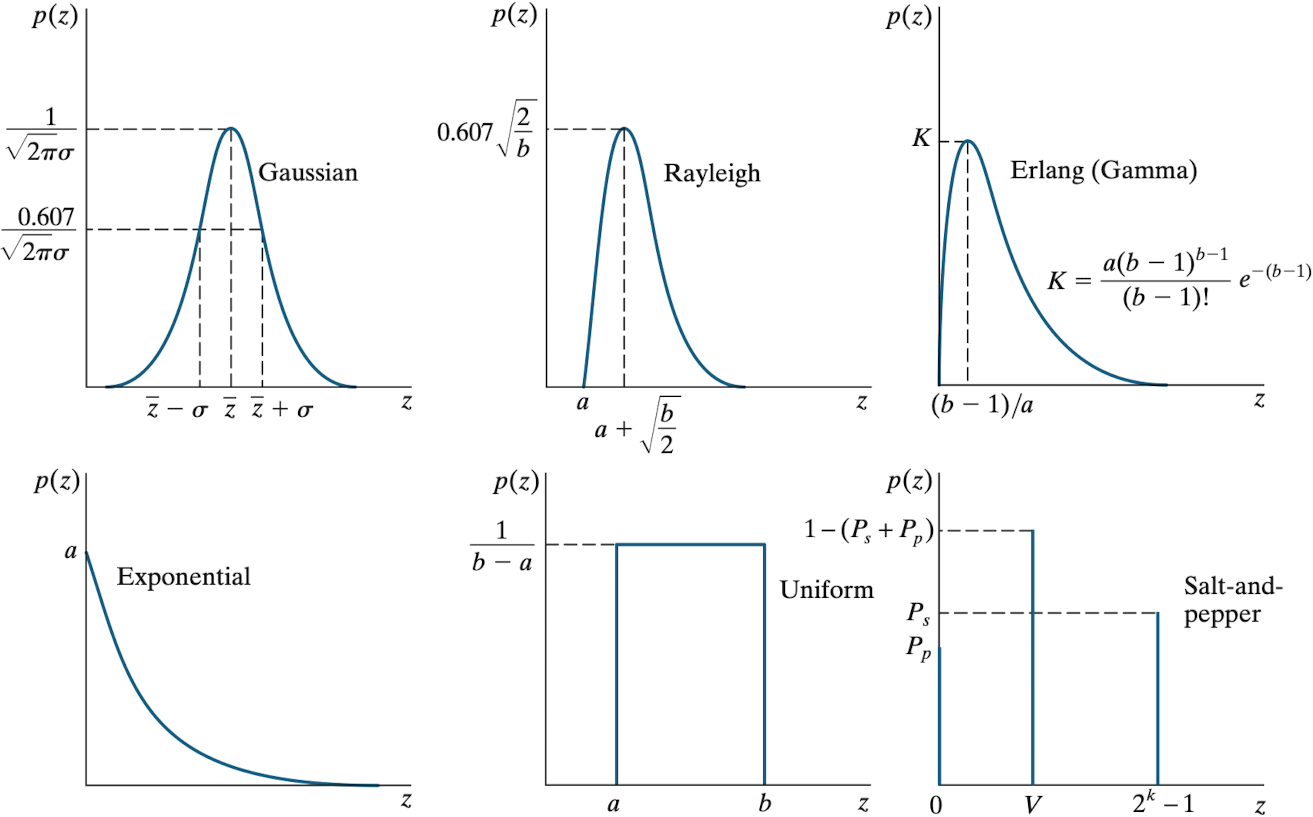
\includegraphics[width=\columnwidth]{noise-models.png}
\end{figure}

이미지 획득 과정에서 노이즈가 생김. digitization에서는 CCD의 한계로 인해 무조건 노이즈가 생김. 흔하게 생기는 노이즈는 white noise. white noise는 모든 주파수 특성이 균일하게 나타나는 노이즈. 주파수 특성을 보면 모든 주파수가 균등한 분포를 가진다. 주기성을 가지는 periodic noise의 반대.

\textbf{Gaussian noise}:
$$p(z) = {1 \over \sqrt{2\pi}\sigma} e^{-(z - \mu)^2/2\sigma^2}$$
$\eta$를 샘플링한 걸 $z$라고 했을 때 확률분포함수는 $p(z)$. 노이즈를 샘플링해서 특성을 알아봤더니 샘플의 분포가 가우시안을 따르는 경우. 가우시안 노이즈는 주로 어두울 때 빛이 적어서 생김.

\textbf{Rayleigh noise}:
$$p(z) = \begin{cases} {2 \over b}(z - a)e^{-(z - a)^2 / b} \; \text{for} \; z \geq a \\ 0 \; \text{for} \; z < a \end{cases}$$

Erlang(Gamma) noise, 밝아지기만 하는 Exponential noise, 분포가 균일한 Uniform noise, Impulse(salt-and-pepper) noise도 있음.

\subsection{Restoration}

노이즈를 없애보자. 일반적으로 노이즈는 크게 가우시안과 rayleigh. 둘 다 노이즈 패턴이 zero mean. 항상 밝아지기만 하는 것도, 어두워지기만 하는 것도 아니기 때문에 자기 주변 픽셀들과 평균을 내면 0. 그래서 나온게 mean filter.

\textbf{Mean filter}: 노이즈 분포가 가우시안일 때는 평균값을 원본 이미지 $\hat{h}$라고 생각할 수 있음. 즉, 가우시안 노이즈에서 $\eta$의 평균은 0(zero-mean). 이런 경우에는 mean filter를 쓸 수 있다. 산술/기하 평균 필터는 가우시안이나 uniform 노이즈에 적합.

\bitmz
  \itm 산술평균 필터: $\hat{f}(x, y) = {1 \over mn} \sum_{(s, t) \in S_{xy}} g(s, t)$.
  \itm 기하평균 필터: $\hat{f}(x, y) = [\Pi_{(s, t) \in S_{xy}} g(s, t)]$. 노이즈 중 하나가 0이라면 전체가 0이 됨. 이미지가 전반적으로 어두워짐.
  \itm 조화평균 필터: $\hat{f}(x, y) = {mn \over \sum_{(s, t) \in S_{xy}} {1 \over g(s, t)}}$. 아웃라이어의 영향이 큼. salt 노이즈는 없앨 수 있지만 pepper 노이즈에는 부적합. salt-and-pepper의 경우 평균이 0이 아니므로.
\eitmz

\textbf{Contraharmonic mean filter}:
$$\hat{f}(x, y) = {\sum_{(s, t) \in S_{xy}} g(s, t)^{Q + 1} \over \sum_{(s, t) \in S_{xy}} {g(s, t)^Q}}$$
파라미터 Q를 이용해서 밝기가 한쪽으로 변하는 이미지를 잘 필터링할 수 있다. Q가 커질수록 maximum쪽으로 가는 경향. Q가 작으면 작을수록 minimum으로 간다. 그래서 필터를 적용하면 밝기가 달라짐. 어두운 이미지라면 Q값을 크게 해야. $Q > 0$일 때는 페퍼 노이즈를, $Q < 0$일 때는 솔트 노이즈를 제거.

가우시안이나 uniform 노이즈에는 산술 평균 필터, impulse 노이즈(salt-and-pepper)에는 contraharmonic 필터. 이미지의 노이즈 특성을 고려하지 않고 Q값을 설정하면 필터링이 이상하게 된다.

\textbf{Order-statistics filer}: 순서가 있는 필터. 대표적으로 median filter. salt-and-pepper noise가 posterized되는 느낌으로 개선됨. 아웃라이어를 제외하는 방식으로 노이즈를 제거. median이 아니라 max, min도 할 수 있음. max는 작은 아웃라이어가, min은 큰 아웃라이어가 없어짐. 하지만 검은 선이 얇아지거나(max) 두꺼워지는(min) 문제가 있음. contraharmonic을 Q값에 따라 max, min으로 만들 수 있음. min과 max를 더해서 평균을 내는 midpoint filter도 있음.

\textbf{Alpha-trimmed mean filter}: 여러 노이즈가 섞여 있는 경우 사용. 가령 salt-and-pepper와 가우시안이 조합되어 있다. $d/2$ lowest와 $d/2$ highest gray-level 값을 제거한다.

\textbf{Adaptive filter}: 평균 필터를 쓰면 이미지가 뭉개지는 문제가 있음. 이를 해결하려면 고주파(엣지, 색이 급격히 바뀌는 부분)은 살리고 노이즈만 없애도록 해야 함. 그래서 노이즈의 분포를 이용. 분포의 형태 뿐만이 아니라 산포도($\sigma$)를 사용. 이미지가 좋은 산포를 갖고 있다면 그 범위 밖에 있는 것을 엣지라고 생각해서 살릴 수 있음. 반면 가운데로 몰리는 것들은 노이즈일 가능성이 높다.
$$\hat{f}(x, y) = g(x, y) - {\sigma_\eta^2 \over \sigma_L^2}[g(x, y) - m_L]$$
$\sigma_L^2$를 $w$라고 하면, $g(x, y) - wg(x, y) - wm \therefore g(x, y) = (1 - w) g(x, y) - wm$. $w$만 잘 결정하면 된다. 분포를 봤을 때 노이즈의 분포와 비슷하다면 노이즈라는 것. $\sigma_\eta^2 < \sigma_L^2$라면 노이즈가 아니라 다른 엣지 같은게 있다는 의미니까 $g(x, y)$에 가까운 값을 쓴다. 우연히 $\sigma_\eta^2 = \sigma_L^2$라면 엣지는 없고 노이즈만 잔뜩 있다는 뜻. 0이면 노이즈가 없으므로 $g(x, y)$를 그대로 사용. adaptive filter는 느리다.

\textbf{Adaptive median filter}: 한 픽셀 주변의 median과 min을 본다. $z_{med} - z_{min}$하면 0보다 큼. $z_{med} - z_{max}$는 0보다 작음. 하지만 샘플이 부족하면 그게 아닐 수도. 그러면 윈도우 크기를 키워서 샘플링을 더 해야 한다. 기본 개념은 median 필터. median을 쓰는 이유는 아웃라이어를 제외하고 싶어서. adaptive median은 아웃라이어인지 아닌지 확인하는 것. 일단 아웃라이어가 나올 때까지 찾는다. 그래서 아웃라이어가 나올 때까지 윈도우 크기를 점점 키워간다. salt-and-pepper 노이즈를 없앨 수 있음. median blur처럼 약간 부드럽게 되는 효과가 있음. 그럼에도 선이 두꺼워지거나 얇아지는 문제는 해결된다.

\subsection{Periodic Noise Reduction}

periodic noise는 일정한 주기를 가진 주파수 특성.

\textbf{Bandreject filter}: 특정 대역을 제외하는 필터. bandpass는 특정 대역만 통과시키는 것. 반지름 $D_0$를 이용해 범위를 설정한다. $H(u, v)$는 $D(u, v) < D_0 - {W \over 2}$라면 1, $D_0 - {W \over 2} \leq D(u, v) \leq D_0 + {W \over 2}$라면 0, $D(u, v) > D_0 + {W \over 2}$라면 1. $D(u, v) = [(u - M / 2)^2 + (v - N / 2)^2]^{1/2}$.

\textbf{Notch reject filter}: 대역 전체가 노이즈는 아닐 수 있음. 그래서 대역의 일부만 지운다. 반대로 notch pass도 가능.

\subsection{Linear, Position-Invariant Degradations}

$g(x, y)$는 $H$라는 함수가 적용이 되고, 여기에 노이즈 $\eta$가 붙어서 만들어진 것. 여기서 $H$는 degradation function. $H$가 리니어하다고 할 때는 additivity, homogeneity, position invariant를 만족할 때.

\bitmz
  \itm Additivity: $H[f_1(x, y) + f_2(x, y)] = H[f_1(x, y)] + H[f_2(x, y)]$
  \itm Homogeneity: $H[af_1(x, y)] = aH[f_1(x, y)]$
  \itm Position invariant: $H[f(x - \alpha, y - \beta)] = g(x - \alpha, y - \beta)$
\eitmz

position invariant는 어느 위치에 degradation을 하든 결과가 똑같다는 것. ($H$가 위치에 따라 변하지 않는다.) 이미지 위치에 상관없이 똑같이 degradation이 일어나는 경우. 예를 들면 카메라가 흔들렸을 때.

\textbf{Point spread function}: degradation function이 linear하다면 point spread function으로 모델링할 수 있음. $g(x, y) = H[f(x, y)] = H[\int_{-\infty}^{\infty} \int_{-\infty}^{\infty} f(\alpha, \beta) \delta(x - \alpha, y - \beta) d\alpha d\beta]$. 한 포인트에서만 값을 가지는 함수 $\delta$를 spread 시켜서 $h$ 함수를 만든다. 즉, $\delta$를 degradation한 것을 통째로 $h$로 표현. 따라서 $h(x, \alpha, y, \beta) = H[\delta(x - \alpha, y - \beta)$. 이때 degradation function을 컨볼루션으로 표현할 수 있음: $g(x, y) = h(x, y) \ast f(x, y) + \eta(x, y)$.

\subsection{Estimating the Degradation Function}

Degradation function을 추정하려면: $H_s(u, v) = G_s(u, v) / \hat{F_s}(u, v)$. 이때 원본 이미지가 딱 한 점만 찍혀 있는 것이라면 $\hat{F_s}$가 상수 $A$로 표현됨. 따라서 $G_s$만 측정하면 된다.

\textbf{Atmospheric turbulence}: 대기, 와류로 인해 빛의 방향이 흐트러진다. $H(u, v) = e^{-k(u^2 + v^2){5 \over 6}}$. 분포를 결정하는 k값을 적절히 조절해야. 작을수록 선명해짐.

\textbf{Motion Blur}: $g(x, y) = \int_0^T f[x - x_0(t), y, - y_0(t)]dt$. 모션 블러 역시 point blur function. 카메라가 한방향으로만 흔들린 경우에 쓸 수 있음.

\subsection{Inverse Filtering}

\begin{figure}[h]
  \centering
  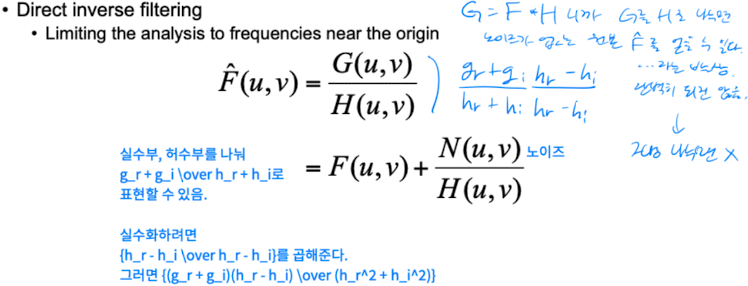
\includegraphics[width=\columnwidth]{inverse.png}
\end{figure}

흔들린 사진을 원본으로 되돌린다. $G = F \ast H$이므로 $G$를 $H$로 나누면 노이즈가 없는 원본 $\hat{F}$를 얻을 수 있지 않을까? (사실 노이즈 $N$의 영향을 고려해야 함)
$$\hat{F}(u, v) = {G(u, v) \over H(u, v)} = F(u, v) + {N(u, v) \over H(u, v)}$$
하지만 그냥 이렇게 하면 분모가 작아져서 잘 안 된다. $H$를 $G$의 일부분에만 나눠서 고주파를 제외하거나 더 포함시켜야. (이미지 중심으로 갈수록 저주파) 하지만 고주파를 과하게 포함하면 분모가 0에 가까워져서 이미지가 망가짐.

\subsection{Minimum Mean Square Error Filtering}

\begin{figure}[h]
  \centering
  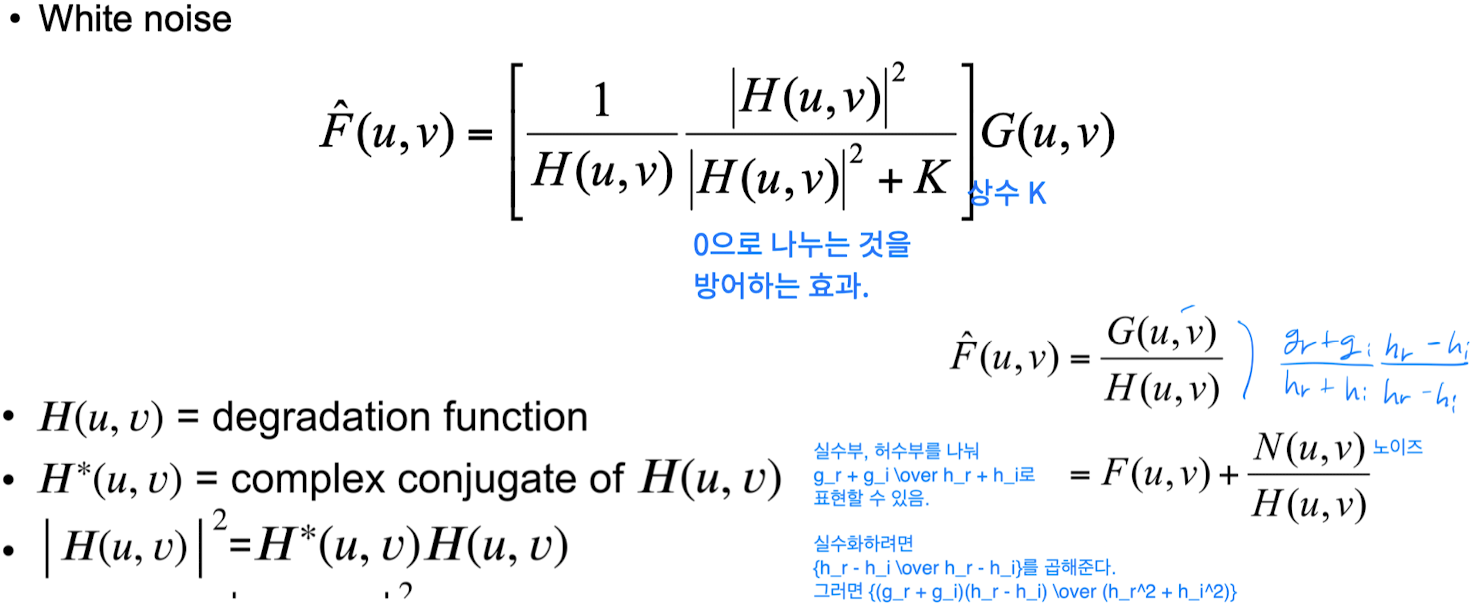
\includegraphics[width=\columnwidth]{wiener.png}
\end{figure}

원본과 추정 이미지 차이 제곱의 합을 최소화하는 것. 분모 $H$가 0에 가까워지면 분자 $H^2$이 더 빠르게 0에 가까워짐으로써 0으로 나누는 효과를 방어한다.

\section{Bilateral and Image Guided Filters}

가우시안으로 노이즈를 없앨 때 치명적인 문제: 노이즈는 없어지지만, 과하게 쓰면 가우시안이 새로운 degradation function으로 작동하기 시작. 이미지를 large-scale(구조, 전체적인 윤곽), small-scale(질감, 디테일)로 구분해보자.

가우시안 블러된 이미지를 복원할 때 저주파를 줄이고 고주파를 강조하는 방법을 시도할 수 있음. unsharpen 필터링과 비슷. 하지만 나이브하게 고주파를 강조하면 fine detail도 같이 강조되면서 이미지가 부자연스러워짐. 블러하면서 엣지가 함께 블러되고, 이로 인해 halo(후광)이 생기는 것.

\begin{figure}[h]
  \centering
  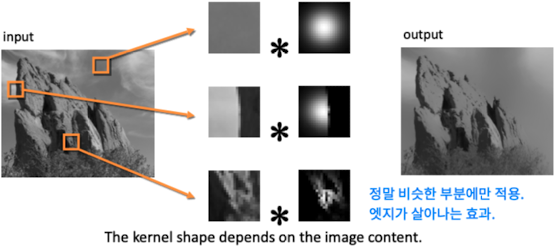
\includegraphics[width=\columnwidth]{bilateral-1.png}
\end{figure}

가우시안 블러를 하면 박스 필터와 달리 결과물에 격자 무늬가 보이는 것을 방지할 수 있다. 하지만 전반적으로 어두워질 수 있음. bilateral 필터는 이때 가우시안과 달리 다른 요소라고 판단된 것을 필터에서 제외시킴으로써 엣지가 블러되지 않도록 살린다.

\begin{figure}[h]
  \centering
  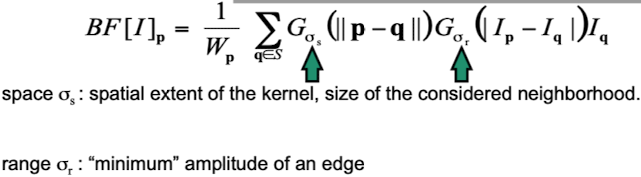
\includegraphics[width=\columnwidth]{bilateral-2.png}
\end{figure}

$\sigma_r$과 $\sigma_s$ 값에 따라 조정가능. $\sigma_r$이 커질수록 엣지가 점점 흐려지고(무한대면 가우시안 블러와 같음), $\sigma_s$가 커질수록 질감(fine detail)이 점점 사라진다. 결과물이 posterized되는 느낌.

단점도 있다: bilateral은 linear하지 않고, 따라서 separable하지도 않음. FFT를 쓰려면 모든 커널이 같은 형태여야 하는데, 그렇지 않으니 FFT도 못씀. 연산량이 많고 느리다.

\section{Color Image Processing}

\subsection{Color Fundamentals}

Radiance: 광원에서 방출되는 에너지의 총량, 와트로 표현. Luminance: 광원으로부터 관측자에게 도달하는 에너지의 양. 루멘스로 측정, 관측자 입장. Brightness: 상대적, 주관적으로 표현되는 밝기의 정도.

Trichromacity-Based Color Model: 원색 3개로 모든 색상을 만들 수 있음. 이렇게 정의한 빛의 삼원색이 RGB. 하지만 실제로는 RGB로 모든 색을 표현할 수가 없다. 이를 표현하기 위한 색공간이 XYZ. 하지만 실제로 만들 수는 없기 때문에 색을 표현하는 방법일뿐. XYZ를 표현하려면 결국 RGB로 바꿔야 한다.

RGB는 빛을 발광하는 대상의 색을 표현할 때, CMYK는 빛을 반사하는 대상의 색을 표현할 때 사용. HSI는 사람에게 색을 설명할 때. XYZ는 수치적으로 색을 표현, RGB가 모든 색을 수치적으로 표현하지 못하기 때문에 사용. RGB로 표현할 수 있는 색공간 안에서 어느 범위까지 색을 표현할 수 있는지에 따라 모니터의 색표현력이 결정.

\subsection{Color Models}

색상을 정의하는 표준적인 방법. RGB, CMY(K), HSI 모델이 있음.

\textbf{RGB Color model}: 독립적인 RGB 컬러로 색을 표현. 각 색상의 max 값을 꼭짓점으로 그래프를 그리면 큐브가 만들어짐. 12비트 디스플레이라면 max가 4096.

\textbf{Pixel Depth}: RGB 공간에서 각 픽셀이 색상을 표현하는 데 쓰는 비트수. 풀컬러 이미지는 24비트, (R, G, B) = (8b, 8b, 8b). Safe RGB Colors: 구형 모니터에서도 색 구분이 잘 되도록 만든 색공간. 색이 그대로 표현되지는 않아도, 적어도 다른 색은 다른 색으로 구분 됨.

\textbf{CMY(K) model}: CMY로 색을 표현. 여기에 검은 색을 추가한 이유는, (1) 인쇄할 때 검은색을 만드려면 CMY를 모두 써야 하기 때문에 비용이 많이 드는 문제, (2) CMY를 모두 써도 진짜 검은색을 만들기가 어려움. CMY는 각각이 RGB의 보색이므로, 1에서 RGB를 뺀 것과 같다. (반대로 CMY를 RGB로 변환할 때도 1 - CMY하면 된다.)

HSI model: 인간친화적인 컬러 모델. 인간은 Hue(색상), Saturation(채도, 원색에 가까우면 1이고 흰색에 가까우면 0), Brightness(명도)로 색을 설명함.

\subsection{Pseudo Color Image Processing}

실제 색상과 상관없이 목적에 따라 색을 부여하는 것. Intensity slicing: intensity가 어떤 임계값을 넘으면 다른 색으로 구분. (e.g., 열영상) 슬라이싱 자체가 어떤 임계값을 기준으로 분류한다는 뜻. Hypercube slicing은 맨하탄 거리 사용.

하나의 Gray Level 이미지를 RGB transformation해서 각각의 RGB를 얻음. 입력 이미지를 여러 장 사용할 수도 있음.

\subsection{Full-color Image Processing}

픽셀은 색상 R, G, B로 구성된 벡터. 근데 RGB 채널을 각각 처리하고 합칠 수도 있음.

어떤 컬러 모델을 사용할 것인가? RGB 색상을 밝게 만드려면 각 채널에 $k$를 곱해준다: $s_i = kr_i$. CMY는 RGB로 변환해서 k를 곱하고 다시 CMY로 변환: $s_i = kr_i + (1 - k)$. HSI는 단순히 I 값만 키워주면 된다: $s_3 = kr_3$.

보색을 얻으려면 RGB는 그냥 1에서 빼면 된다. CMYK는 1에서 RGB를 빼서 변환할 수 있음. HSI는 H를 반바퀴 회전시킨다. 즉, 0.5 더해주되, 1보다 커지면 1을 빼준다. 근데 실제로 해보면 둘이 동일하지 않음.

색은 RGB의 비율로 결정된다. 어두운 이미지를 밝게 하기 위해 어두운 부분의 기울기를 가파르게 하는 필터를 적용하면 색이 변하는 문제. 색상의 비율이 달라지면, 상대적으로 비율이 높아서 채도가 강해보이던 색의 채도가 떨어짐. 결과적으로 밝은 부분의 채도가 낮아짐. 가령 CMYK에서 푸른 색이 강하면 마젠타를 높이고, 보라색이 강하면 노랑을 높이는 식으로 보정 가능.

컬러 이미지에 히스토그램 평탄화를 한다면? RGB 채널별로 각각 평탄화하면 이미지가 망가짐. HSI에서 H와 S는 남겨두고 I만 평탄화하면 밝기만 조정할 수 있다. 실제로는 색감이 조금 바뀌기 때문에 Saturation 조정도 필요.

\subsection{Smoothing \& Sharpening}

흑백 이미지와 마찬가지로 RGB 이미지에서도 neighborhood processing을 할 수 있음. 각 채널별로 spatial filtering을 수행. 스무딩이나 샤프닝을 할 때 채널별로 수행한 것과 HSI의 I에 대해서 수행한 것의 결과가 비슷함.

RGB 공간에서의 범위는? 한 점을 기준으로 주변 색상을 같은 것으로 취급한다. $D(z, a) = ||z - a|| = [(z - a)^T(z - a)]^{1 \over 2}$. 타원을 만들고 싶으면 $C$를 이용해 구체의 방향을 설정할 수 있음. 이를 Mahalanobis distance라고 함: $D(z, a) = [(z - a)^T C^{-1} (z - a)]^{1 \over 2}$

\begin{figure}[h]
  \centering
  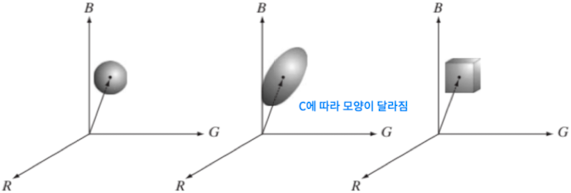
\includegraphics[width=\columnwidth]{rgb-space-range.png}
\end{figure}

이때 $(z - a)^T$는 열벡터를 행벡터로 바꾼 것. 즉, 행벡터와 열벡터를 곱하는 것, 여기서는 결국 $(z - a)$를 제곱해서 루트 씌운다는 의미.

Edge detection: RGB를 각각하면 안 됨. 미분값은 하나만 써야 하니까. 그래서 각 채널을 미분하고 더한 값을 사용.
$$
\begin{aligned}
  g_{xx} &= {\partial R \over \partial x} + {\partial G \over \partial x} + {\partial B \over \partial x} \\
  g_{yy} &= {\partial R \over \partial y} + {\partial G \over \partial y} + {\partial B \over \partial y}
\end{aligned}
$$

\section{Morphological Image Processing}

SE(Structuring Element): 기준 픽셀 하나와 이웃한 픽셀들을 포함한 요소. 이미지의 모든 픽셀과 SE를 비교하며 특정 기준으로 필터링을 수행한다.

\textbf{Erosion}: $A \circled{-} B = \{z | (B)z \subseteq A\}$. SE의 모든 요소를 포함하는 픽셀만 살린다.

\textbf{Dilation}: $A \circled{+} B = \{z | (B)z \cap A \neq \emptyset\}$. SE가 포함하는 모든 픽셀을 살린다.

erosion과 dilation은 duality를 만족: $(A \circled{-} B)^c = A^c \circled{+} B^c$, $(A \circled{+} B)^c = A^c \circled{-} B^c$.

\textbf{Opening}: $A \circ B = (A \circled{-} B) \circled{+} B$. 애매하게 이어진 부분을 끊고 경계를 부드럽게 만든다. 항상 결과가 원본보다 작아지고, 오프닝을 여러 번 해도 한 번한 것과 결과가 같다.

\begin{figure}[h]
  \centering
  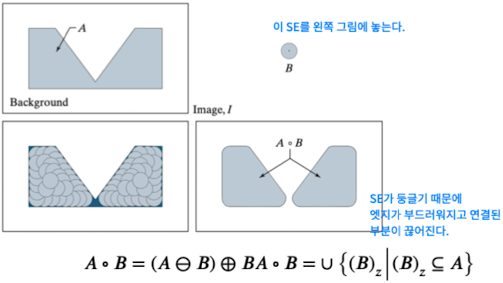
\includegraphics[width=\columnwidth]{opening.png}
\end{figure}

\textbf{Closing}: $A \cdot B = (A \circled{+} B) \circled{-} B$. 떨어진 부분을 잇고 작은 구멍을 채운다. 결과가 원본보다 커지고, 클로징을 여러 번 해도 한 번한 것과 결과가 같다.

\begin{figure}[h]
  \centering
  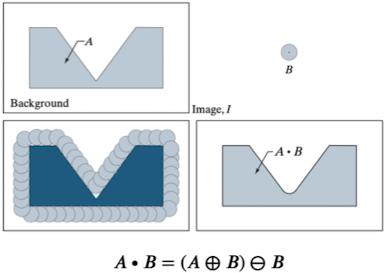
\includegraphics[width=\columnwidth]{closing.png}
\end{figure}

opening과 closing은 duality를 만족: $(A \circ B)^c = (A^c \cdot B^c)$를 증명하면:
$$
\begin{aligned}
(A \circ B)^c &= ((A \circled{-} B) \circled{+} B)^c \\
&= (A \circled{-} B)^c \circled{-} B^c \\
&= (A^c \circled{+} B^c) \circled{-} B^c \\
&= A^c \cdot B^c
\end{aligned}
$$
$(A \cdot B)^c = (A^c \circ B^c)$를 증명하면:
$$
\begin{aligned}
(A \cdot B)^c &= ((A \circled{+} B) \circled{-} B)^c \\
&= (A \circled{+} B)^c \circled{+} B^c \\
&= (A^c \circled{-} B^c) \circled{+} B^c \\
&= A^c \circ B^c
\end{aligned}
$$

\textbf{Hit-or-Miss Transformation(HMT)}: $I \bigoast B$. SE를 다양하게 활용해보자는 발상. SE와 동일한 형태 요소의 중앙점만 남는다. (e.g., SE를 A 모양으로 만들면 이미지에서 A를 찾는 OCR 가능.)

\begin{figure}[h]
  \centering
  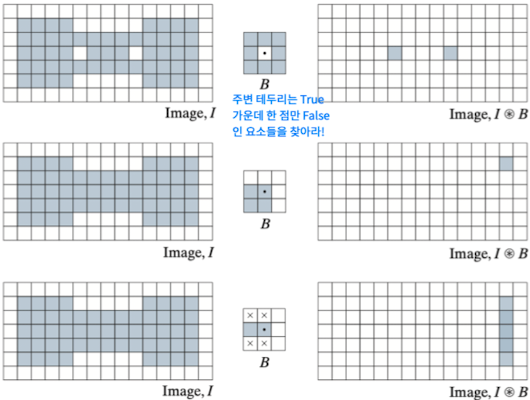
\includegraphics[width=\columnwidth]{hmt.png}
\end{figure}

boundary extraction에도 사용할 수 있음. 자신은 True고, 주변에 False가 있는 경우 inner boundary로 정의. outer boundary는 그 반대.

\begin{figure}[h]
  \centering
  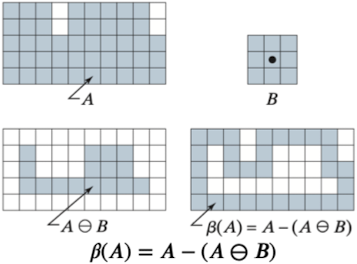
\includegraphics[width=\columnwidth]{boundary-extraction.png}
\end{figure}

같은 원리로 색상 채우기도 가능. 처음 한 seed에서 시작해 SE와 $A^c$ 이미지를 교집합하며 더 이상 변화가 없을 때까지 recursive하게 진행.

\begin{figure}[h]
  \centering
  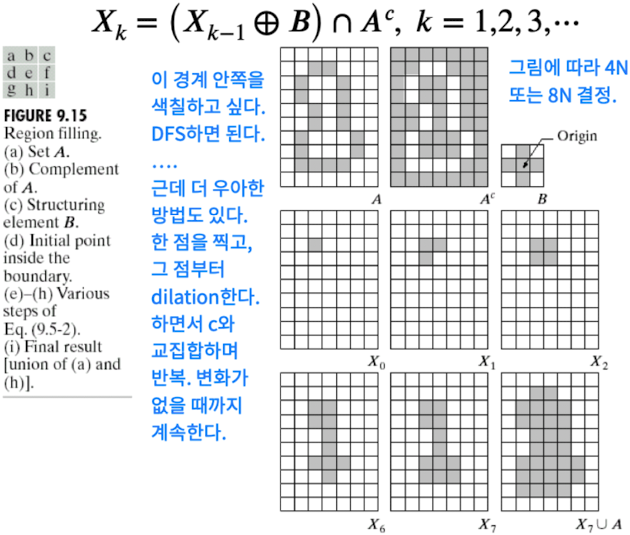
\includegraphics[width=\columnwidth]{region-filling.png}
\end{figure}

\textbf{Extraction of Connected Components}: $X_k = (X_{k-1} \bigoplus B) \cap A$. 경로가 존재하는 컴포넌트. True인 픽셀만 거쳐서 도달할 수 있는가? $X$의 앞 결과를 이용해 iterative하게 수행한다.

\textbf{Thining}: $A \bigotimes B = A - (A \bigotimes B) = A \cap (A \bigoast B)^c$. 뼈대만 남기고 싶을 때.

\textbf{Thickening}: $A \bigodot B = A \cup (A \bigoast B)$. 뼈대에 살을 붙일 때.

\textbf{Morphological Reconstruction}: 마스크 안쪽에서만 탐색하는 것(thresholding). 찾고자하는 모양을 SE로 erosion하면 해당 모양이 있는 위치에만 점이 찍혀서 남음. 그렇게 얻은 각 점을 seed로 마스크 범위 내에서 이터레이티브하게 region을 키워나간다(마스크와 교집합).

\textbf{Gray-Scale Morphology}: thresholding을 하지 않고도 morphological operation을 할 수 있음.

\bitmz
  \itm Erosion: $[f \circled{-} b](x, y) = min_{(s, t) \in b}[f(x + s, y + t)]$
  \itm Dilation: $[f \circled{-} b](x, y) = max_{(s, t) \in b}[f(x + s, y + t)]$
  \itm Duality: $(f \circled{-} b)^c = (f^c \bigoplus \hat{b})$, $f$의 complement는 max에서 값을 뺀 것과 같음.
\eitmz

\textbf{Morphological Gradient}: morphological operation으로 급격하게 밝기가 변하는 부분, 엣지를 찾아본다. $g = (f \circled{+} b) - (f \circled{-} b)$.

\textbf{Top-hat Transformation}: 배경을 없애준다. $T_{hat}(f) = f - (f \circ b)$. 비전 전처리에 사용 가능.

\section{Image Compression}

이미지의 정보에 비해 데이터가 과할 때가 있다. 데이터는 정보를 전달하는 수단. 최대한 많은 정보를 더 적은 데이터로 표현하는 것이 압축. 손실과 압축률에는 트레이드오프가 있음. (lossy vs lossless) 실제로 사용되는 대부분의 압축은 손실을 감수하므로 lossy하다.

압축률: 압축 전 비트가 $n_1$, 압축 후 비트가 $n_2$라면, 압축률 $C_R = {n_1 \over n_2}$. compression ratio가 10이면 1/10으로 줄었다는 것. 압축 후 불필요한 데이터가 얼마나 제거되었는가(data redundancy): $R_D = 1 - {1 \over C_R}$. 다양한 종류의 데이터 redundancy가 있음.

\textbf{Coding redundancy}: 픽셀마다 다른 비트를 사용할 수 있을까? $k$번째 그레이 레벨이 $r_k$만큼의 비트를 사용한다고 가정. 검은색은 1비트, 밝아질수록 더 많은 비트를 쓴다. 평균 이미지 비트수는 $NML_{avg} = \sum l(r_k)P(r_k)$. 이미지가 통째로 검은색이면 $N \times M \times 1$. coding redundancy를 줄이는 과정은 entropy encoding.

\begin{figure}[h]
  \centering
  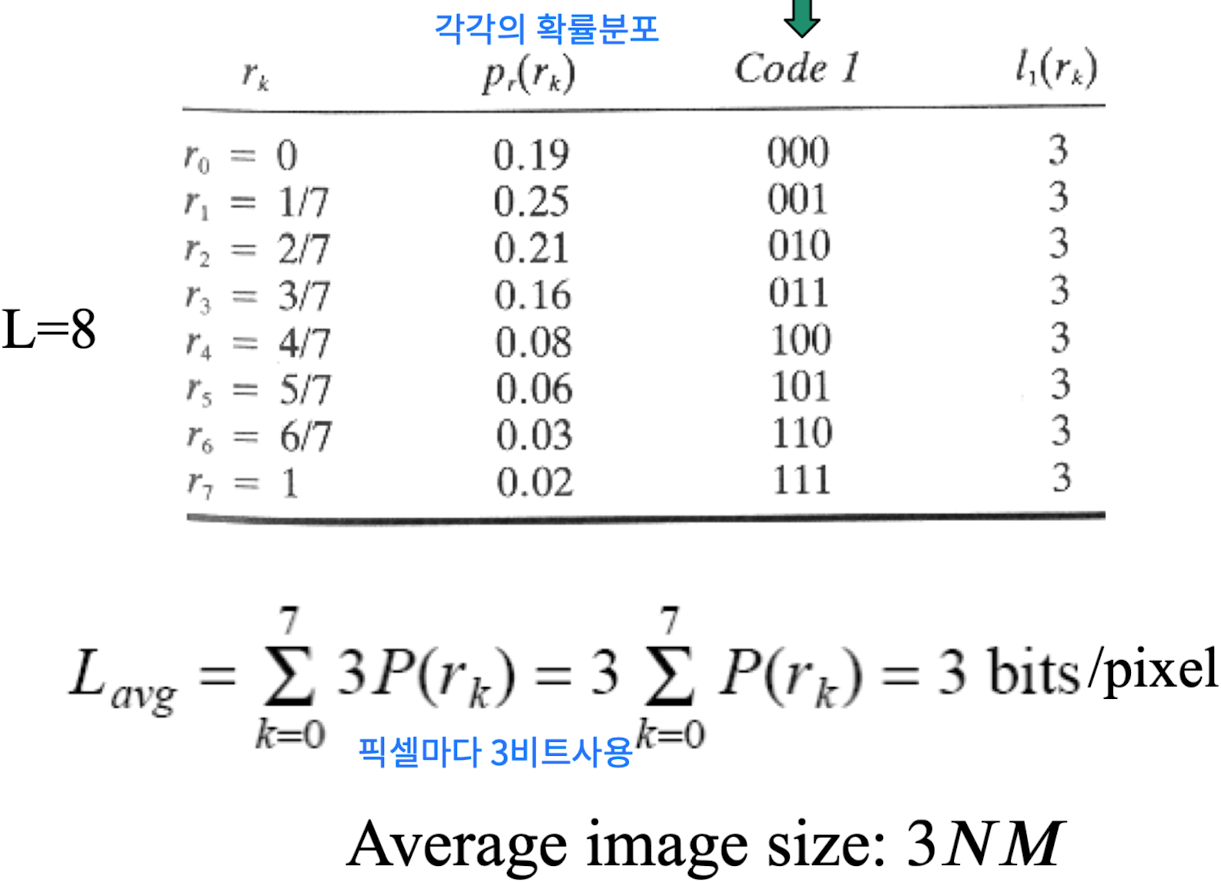
\includegraphics[width=\columnwidth]{coding-redundancy-fixed.png}
\end{figure}

\begin{figure}[h]
  \centering
  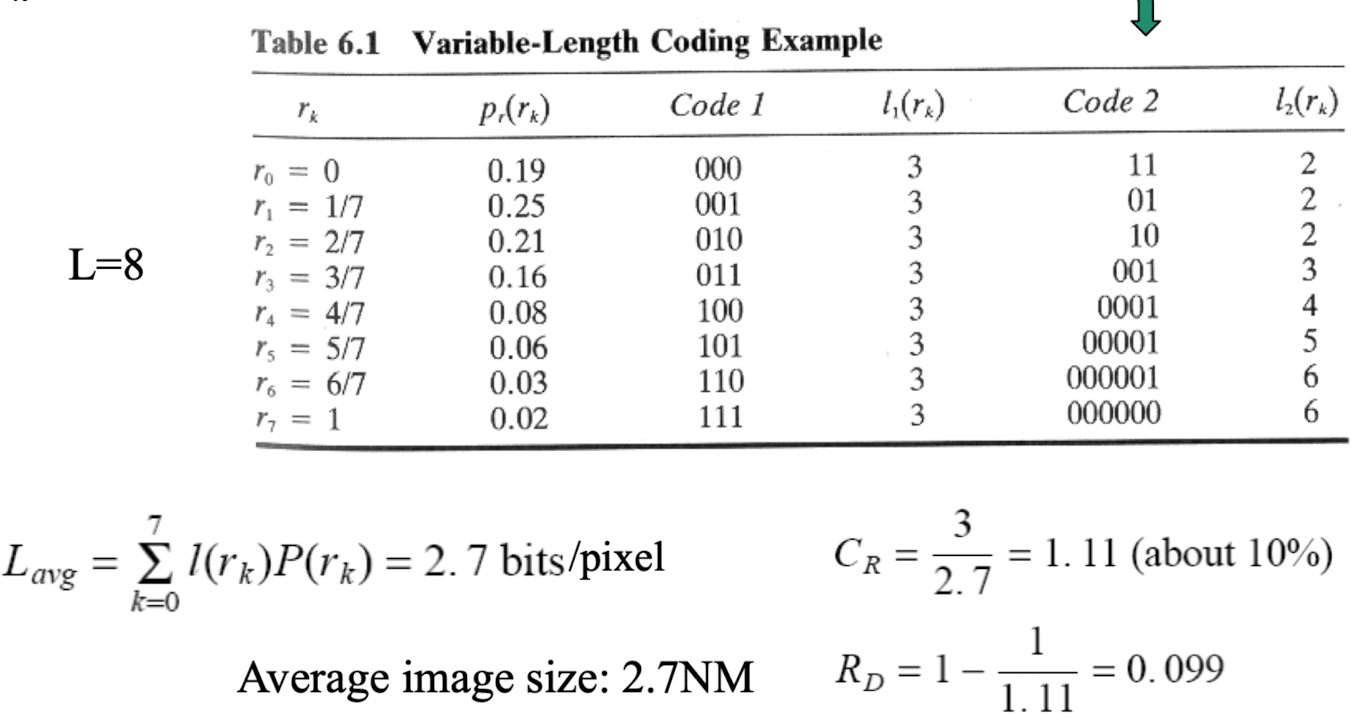
\includegraphics[width=\columnwidth]{coding-redundancy-variable.png}
\end{figure}

\textbf{Interpixel redundancy}: 밝은 것은 종이고, 까만 것은 글씨. 즉, 흑백 이미지라면 명암을 제거함으로써 같은 정보를 전달하면서도 데이터를 줄일 수 있다. 회색을 지우고 흰색과 검은색으로 모든 것을 표현할 수 있다.

\subsection{Symbolic Encoding}

\textbf{Huffman Coding}: coding redundancy는 같은 정보를 전하는데 구성을 바꿔서 양을 줄일 수 있음. 데이터의 빈도수(확률)에 따라 이진 코드를 할당하고 인코딩하는 알고리즘. 모든 데이터를 인코딩하므로 lossless하다. 디코딩하려면 인코딩할 때 만든 트리가 필요함. 가령 \code{01010/011/1/1/00}을 디코딩하면, $a_3 a_1 a_2 a_2 a_6$:

\begin{figure}[h]
  \centering
  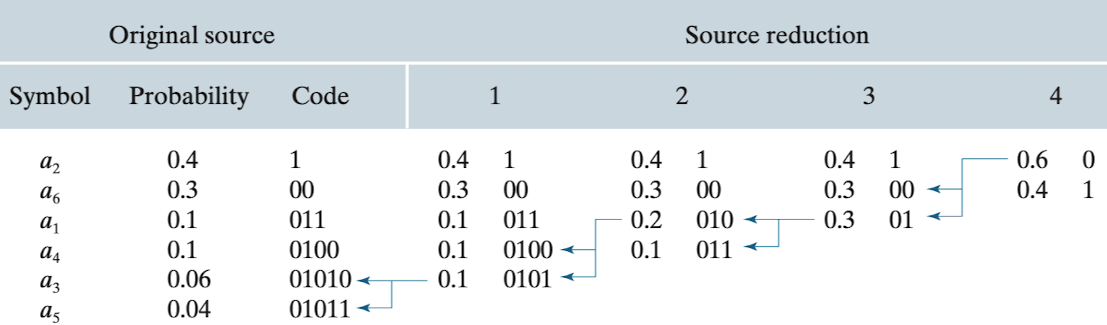
\includegraphics[width=\columnwidth]{huffman-coding.png}
\end{figure}

이때 $L_{avg} = (0.4)(1) + (0.3)(2) + (0.1)(3) + (0.1)(4) + (0.06)(5) + (0.04)(5) = 2.2bits/pixel$. 6개 심볼을 사용하므로 단순 이진 인코딩했다면 3비트($111 = 7$)가 필요함.

\textbf{LZW(Lempel-Ziv-Welch) Coding}: 딕셔너리를 활용. 데이터를 읽으며 자주 등장하는 데이터를 딕셔너리에 등록한다. 데이터가 올때마다 딕셔너리를 만들어나갈 수 있기 때문에 허프만과 달리 읽는 쪽에서 완성된 딕셔너리를 유지할 필요가 없음. 모든 데이터가 한 번은 딕셔너리에 등록되므로 lossless. 허프만도 그렇고 이것도 중간에 한 비트가 깨지면 그 뒤로는 모두 망가져버림.

\textbf{RLC(Run-Length Coding)}: 반복되는 일련의 심볼을 개수와 함께 저장. 가령 \code{aaabbbbbbccaa}는 $(a, 3), (b, 6), (c, 2), (a, 2)$. 중복된 심볼도 새 튜플로 저장하므로 lossless.

\subsection{Mapping and Quantization}

앞서 본 인코딩은 엔트로피가 낮은 경우에만 효과가 있음. 즉, 정보량이 적어야 함. 아예 엔트로피를 줄여보면 어떨까? 손실이 일어나는 lossy compression을 한다. 단, 사람이 봤을 때 구분할 수 있는 수준으로만 손실이 있어야 함. Objective Fidelity Criteria: 손실을 객관적으로 측정하기 위한 지표.

\textbf{DCT}: DFT와 비슷하지만 손실이 적은 압축이 가능. 블록 단위로 주파수를 분할해 각 블록에 독립적으로 적용. 낮은 주파수 대역에 있는 중요한 정보를 유지하면서 고주파 성분을 제거함으로써 압축을 가능하게 함.

\textbf{JPEG}: (1) 입력 이미지를 8$\times$8 블록으로 쪼갠다. (블록 크기에 따라 에러가 달라짐.) (2) 그레이 레벨을 [-128, 127] 범위로 조정하고, (3) DCT를 적용한다. (4) DCT의 결과로 얻은 coefficients를 quantize한다. (quantization table은 JPEG에서 정의해놓음. 테이블의 숫자가 작으면 압축률이 낮아짐.)

이 결과를 지그재그순으로 저장하는데, 이렇게함으로써 주파수 성분이 거의 변화하지 않는 영역(뒤쪽)의 데이터를 줄일 수 있다. 읽을 때는 가장 먼저 quantization table을 읽고, 디코딩한 뒤 지그재그로 읽는다.

\begin{figure}[h]
  \centering
  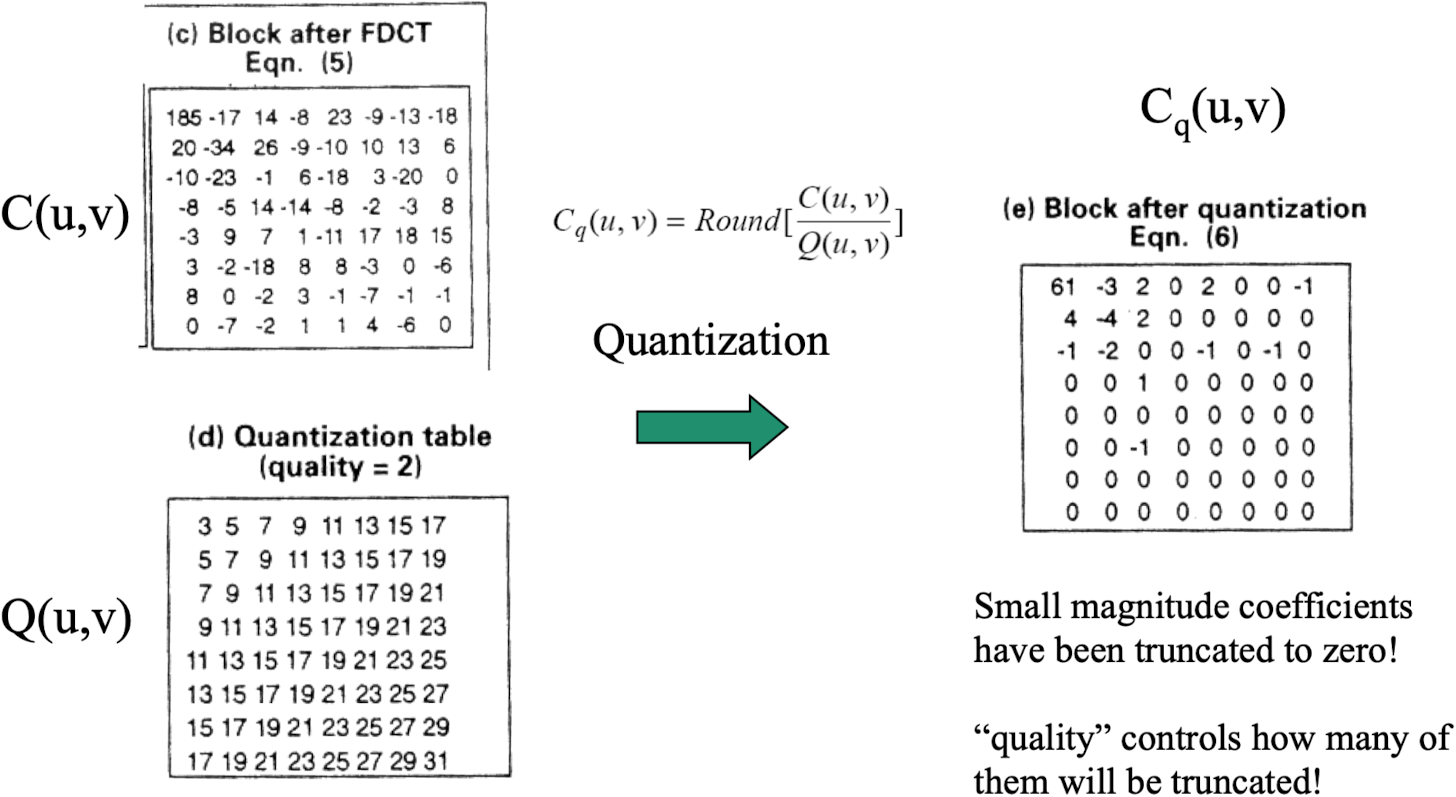
\includegraphics[width=\columnwidth]{jpeg-quantization.png}
\end{figure}

\textbf{Chroma Subsampling}: 컬러는 어떻게 압축? RGB로 하면 안됨. 세상의 평균은 회색이므로 원점이 회색인 YCrCb 색공간 사용해야. 여기서 Y는 휘도, CrCb는 색차(Chroma). 사람은 밝기 차에는 민감하지만 색상 차에는 상대적으로 둔감하다. 따라서 Y에는 많은 비트를 사용하고, CrCb에는 적은 비트를 사용 가능. JPEG은 4:2:0 subsampling을 채택, 컬러를 1/4만 사용함으로써 압축한다.

\textbf{Progressive JPEG}: 이미지를 좌에서 우로, 상에서 하로 single scan하면 이미지가 보여지는 데 너무 오랜 시간이 걸린다. progressive JPEG는 일단 DC만 인코딩해서 흐린 이미지를 보여주고, 여러번 디코딩해서 점점 이미지가 잘 보이도록 한다.
